% SC1004 Chapter 4: Vector Spaces (0->100 ground-up)
\chapter{Vector Spaces}
\label{ch:vectorspaces}

\begin{quote}
\emph{``A vector space is any place where arrows still make sense.''} We abstract $\mathbb{R}^n$ to uncover spaces of matrices, polynomials, signals, and images --- all governed by the same eight rules.
\end{quote}

\noindent\fbox{\parbox{\dimexpr\linewidth-2\fboxsep-2\fboxrule}{%
\textbf{From zero: axioms after examples.} We have lived in $\mathbb{R}^n$ for three chapters. Now we ask what makes it tick, write the rules down, and test which other collections obey them. Every axiom is motivated by a picture or a failure.}}
\vspace{0.4em}

\section*{Learning Outcomes}
After this chapter you will be able to:
\begin{enumerate}[label=(L\arabic*)]
    \item state the eight vector-space axioms and test a set against them;
    \item recognise subspaces and verify them via the subspace test;
    \item describe column space, null space, row space, and their relations;
    \item decide membership in a span and express vectors as combinations;
    \item connect subspaces to solutions of $A\mathbf{x}=\mathbf{b}$ and $A\mathbf{x}=\mathbf{0}$.
\end{enumerate}

% ============================================================
\section{Why Abstract?}
\label{sec:why-abstract}
In $\mathbb{R}^n$ we add arrows tip-to-tail and stretch them. But we also add \emph{polynomials} $(p+q)(x)=p(x)+q(x)$, \emph{matrices}, \emph{audio signals} (add waveforms, scale volume), and \emph{RGB images}. Each supports the same two operations. Rather than prove everything four times, we isolate the common rules.

\section{The Axioms}
\label{sec:axioms}
A \emph{vector space} over $\mathbb{R}$ is a set $V$ with addition $+$ and scalar multiplication $\cdot$ satisfying, for all $\mathbf{u},\mathbf{v},\mathbf{w}\in V$, $c,d\in\mathbb{R}$:
\begin{enumerate}[label=(V\arabic*)]
    \item $\mathbf{u}+\mathbf{v}\in V$ (closure under $+$),\quad $c\mathbf{u}\in V$ (closure under scaling);
    \item $\mathbf{u}+\mathbf{v}=\mathbf{v}+\mathbf{u}$; $(\mathbf{u}+\mathbf{v})+\mathbf{w}=\mathbf{u}+(\mathbf{v}+\mathbf{w})$;
    \item there exists $\mathbf{0}\in V$ with $\mathbf{v}+\mathbf{0}=\mathbf{v}$;
    \item for each $\mathbf{v}$ there is $-\mathbf{v}$ with $\mathbf{v}+(-\mathbf{v})=\mathbf{0}$;
    \item $c(\mathbf{u}+\mathbf{v})=c\mathbf{u}+c\mathbf{v}$;\; $(c+d)\mathbf{v}=c\mathbf{v}+d\mathbf{v}$;
    \item $c(d\mathbf{v})=(cd)\mathbf{v}$;\; $1\mathbf{v}=\mathbf{v}$.
\end{enumerate}
Elements of $V$ are called \emph{vectors} even when they look like matrices or functions.

\begin{figure}[h]
\centering
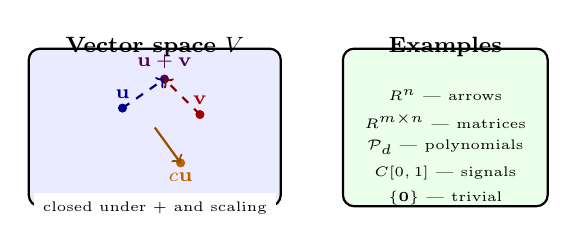
\begin{tikzpicture}[scale=0.82,every node/.style={font=\scriptsize}]
  \node[draw,thick,rounded corners=4pt,fill=blue!8,minimum width=3.2cm,minimum height=2.0cm] (V) at (0,0) {};
  \node[font=\footnotesize\bfseries] at (0,1.25) {Vector space $V$};
  \fill[blue!55!black] (-0.5,0.3) circle (2pt) node[above] {$\mathbf{u}$};
  \fill[red!65!black] (0.7,0.2) circle (2pt) node[above] {$\mathbf{v}$};
  \fill[violet!65!black] (0.15,0.75) circle (2pt) node[above] {$\mathbf{u}+\mathbf{v}$};
  \draw[->,thick,blue!50!black,dashed] (-0.5,0.3)--(0.15,0.75);
  \draw[->,thick,red!50!black,dashed] (0.7,0.2)--(0.15,0.75);
  \fill[orange!75!black] (0.4,-0.55) circle (2pt) node[below] {$c\mathbf{u}$};
  \draw[->,thick,orange!60!black] (0,0)--(0.4,-0.55);
  \node[font=\tiny,fill=white] at (0,-1.25) {closed under $+$ and scaling};

  \node[draw,thick,rounded corners=4pt,fill=green!8,minimum width=2.6cm,minimum height=2.0cm] at (4.5,0) {};
  \node[font=\footnotesize\bfseries] at (4.5,1.25) {Examples};
  \node[font=\tiny,align=left] at (4.5,0.5) {$\mathbb{R}^n$ --- arrows};
  \node[font=\tiny,align=left] at (4.5,0.1) {$\mathbb{R}^{m\times n}$ --- matrices};
  \node[font=\tiny,align=left] at (4.5,-0.3) {$\mathcal{P}_d$ --- polynomials};
  \node[font=\tiny,align=left] at (4.5,-0.7) {$C[0,1]$ --- signals};
  \node[font=\tiny,align=left] at (4.5,-1.1) {$\{\mathbf{0}\}$ --- trivial};
\end{tikzpicture}
\caption{Left: closure means sums and scalings never leave $V$. Right: diverse examples obeying the same axioms.}
\label{fig:vecspace-closure}
\end{figure}

\begin{example}[Polynomials]
$\mathcal{P}_2=\{a_0+a_1x+a_2x^2:a_i\in\mathbb{R}\}$ is a vector space of dimension $3$ (basis $1,x,x^2$). The set $\{p:p(0)=1\}$ is \emph{not} a subspace (fails $\mathbf{0}$ and closure --- sum has $p(0)=2$).
\end{example}

\begin{example}[Non-example]
The first quadrant $\{(x,y):x\ge0,y\ge0\}\subset\mathbb{R}^2$ is not a vector space: $(1,1)$ is in it but $-(1,1)=(-1,-1)$ is not (fails (V4) and scaling by $-1$).
\end{example}

\section{Subspaces}
\label{sec:subspaces}
\begin{definition}[Subspace]
$W\subseteq V$ is a \emph{subspace} if it is itself a vector space under the same $+$ and $\cdot$. Equivalently (subspace test):
\[
  W\neq\emptyset,\quad \mathbf{u},\mathbf{v}\in W\Rightarrow \mathbf{u}+\mathbf{v}\in W,\quad c\in\mathbb{R},\mathbf{u}\in W\Rightarrow c\mathbf{u}\in W.
\]
In particular $\mathbf{0}\in W$ always.
\end{definition}

\begin{figure}[h]
\centering
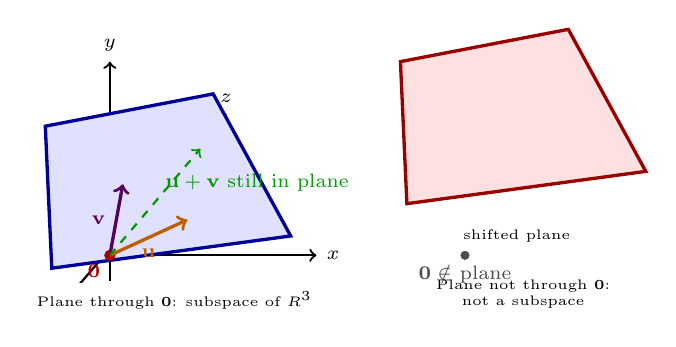
\begin{tikzpicture}[scale=0.82,every node/.style={font=\scriptsize}]
  \draw[->,thick] (-0.4,0)--(3.2,0) node[right] {$x$};
  \draw[->,thick] (0,-0.4)--(0,3.0) node[above] {$y$};
  \draw[->,thick] (-0.6,-0.6)--(1.8,2.2) node[above] {$z$};
  % plane through origin = subspace
  \fill[blue!12] (-0.9,-0.2)--(2.8,0.3)--(1.6,2.5)--(-1.0,2.0)--cycle;
  \draw[very thick,blue!60!black] (-0.9,-0.2)--(2.8,0.3)--(1.6,2.5)--(-1.0,2.0)--cycle;
  \fill[red!70!black] (0,0) circle (2.5pt) node[below left] {$\mathbf{0}$};
  \draw[->,very thick,orange!75!black] (0,0)--(1.2,0.55) node[midway,below] {$\mathbf{u}$};
  \draw[->,very thick,violet!70!black] (0,0)--(0.2,1.1) node[midway,left] {$\mathbf{v}$};
  \draw[->,thick,green!60!black,dashed] (0,0)--(1.4,1.65) node[midway,above right] {$\mathbf{u}+\mathbf{v}$ still in plane};
  \node[font=\tiny,fill=white] at (1.0,-0.7) {Plane through $\mathbf{0}$: subspace of $\mathbb{R}^3$};

  \begin{scope}[xshift=5.5cm]
    \fill[red!12] (-0.9,0.8)--(2.8,1.3)--(1.6,3.5)--(-1.0,3.0)--cycle;
    \draw[very thick,red!60!black] (-0.9,0.8)--(2.8,1.3)--(1.6,3.5)--(-1.0,3.0)--cycle;
    \fill[gray!60!black] (0,0) circle (2pt) node[below] {$\mathbf{0}\notin$ plane};
    \node[font=\tiny,fill=white] at (0.8,0.3) {shifted plane};
    \node[font=\tiny,align=center] at (0.9,-0.6) {Plane not through $\mathbf{0}$:\\not a subspace};
  \end{scope}
\end{tikzpicture}
\caption{Left: a subspace must contain $\mathbf{0}$ and be closed (plane through origin). Right: a translate fails the test.}
\label{fig:subspace-plane}
\end{figure}

\section{Four Fundamental Subspaces of a Matrix}
\label{sec:four-subspaces}
For $A\in\mathbb{R}^{m\times n}$:
\begin{itemize}
    \item \textbf{Column space} $\mathcal{C}(A)=\{A\mathbf{x}:\mathbf{x}\in\mathbb{R}^n\}\subseteq\mathbb{R}^m$ --- all $\mathbf{b}$ for which $A\mathbf{x}=\mathbf{b}$ is solvable. Span of the columns.
    \item \textbf{Null space} $\mathcal{N}(A)=\{\mathbf{x}:A\mathbf{x}=\mathbf{0}\}\subseteq\mathbb{R}^n$ --- homogeneous solutions (Ch.~3). Always a subspace.
    \item \textbf{Row space} $\mathcal{C}(A^T)\subseteq\mathbb{R}^n$ --- span of the rows.
    \item \textbf{Left null space} $\mathcal{N}(A^T)\subseteq\mathbb{R}^m$.
\end{itemize}
$\mathcal{C}(A)$ and $\mathcal{N}(A^T)$ live in $\mathbb{R}^m$; $\mathcal{N}(A)$ and $\mathcal{C}(A^T)$ in $\mathbb{R}^n$. Row operations preserve $\mathcal{N}(A)$ and row space but change $\mathcal{C}(A)$ --- a common pitfall.

\begin{example}[Membership]
Is $\mathbf{b}=[1,2,3]^T$ in $\mathcal{C}(A)$ for $A=\begin{bmatrix}1&2\\2&4\\3&6\end{bmatrix}$? Second column is $2\times$ first, so $\mathcal{C}(A)=\operatorname{span}\{[1,2,3]^T\}$. Since $\mathbf{b}=1\cdot[1,2,3]^T$, yes. $\mathbf{b}'=[1,0,0]^T$ is not.
\end{example}

\begin{example}[Python --- null space]
\begin{lstlisting}[language=Python]
import numpy as np
from scipy.linalg import null_space
A = np.array([[1.,2.,1.],[2.,4.,2.],[1.,1.,0.]])
print("rank", np.linalg.matrix_rank(A))
NS = null_space(A)   # orthonormal basis for N(A)
print(NS.T)          # each row is a basis vector
print(A @ NS)        # ~ 0 (up to round-off)
\end{lstlisting}
\end{example}

% ============================================================

% --- Additional depth: Span, sum, and direct sum ---
\section{Span and Spanning Sets}
\label{sec:span-detail}
For $S=\{\mathbf{v}_1,\dots,\mathbf{v}_k\}\subseteq V$, $\operatorname{span}(S)=\{\sum c_i\mathbf{v}_i:c_i\in\mathbb{R}\}$ is the smallest subspace containing $S$ (intersection of all subspaces containing $S$). $S$ \emph{spans} $V$ if $\operatorname{span}(S)=V$. Spanning is the opposite of independence: too many vectors guarantees dependence, too few cannot span.

\begin{theorem}[Spanning test via matrices]
Fix a basis to coordinatize $V\cong\mathbb{R}^n$. Then $S$ spans $V$ iff the matrix with columns $[{\mathbf{v}_i}]$ has rank $n$ (every $\mathbf{b}$ is a combination).
\end{theorem}

\section{Sums and Direct Sums}
\label{sec:sums}
For subspaces $U,W\subseteq V$, $U+W=\{\mathbf{u}+\mathbf{w}:\mathbf{u}\in U,\mathbf{w}\in W\}$ is a subspace; $U\cap W$ is too. The sum is \emph{direct}, $V=U\oplus W$, if $V=U+W$ and $U\cap W=\{\mathbf{0}\}$ --- then every $\mathbf{v}\in V$ has a unique $\mathbf{u}+\mathbf{w}$ decomposition. Example: $\mathbb{R}^3=\text{$xy$-plane}\oplus\text{$z$-axis}$.

\begin{example}[Polynomial split]
$\mathcal{P}_3=\{p:p(0)=0\}\oplus\{ \text{constants}\}$: every $p(x)=a_0+a_1x+a_2x^2+a_3x^3$ uniquely as $(a_1x+a_2x^2+a_3x^3)+a_0$. Dimensions add: $3+1=4=\dim\mathcal{P}_3$.
\end{example}

\section{Coordinates Revisited}
\label{sec:coords-vec}
Fix a basis $B=\{\mathbf{b}_1,\dots,\mathbf{b}_n\}$ of $V$. The map $\mathbf{v}\mapsto[\mathbf{v}]_B\in\mathbb{R}^n$ (coordinates) is a linear isomorphism: it preserves $+$ and scaling and is bijective. So every $n$-dimensional real vector space is ``just'' $\mathbb{R}^n$ in disguise --- but the disguise matters for interpretation (e.g.\ polynomial vs.\ signal).



\begin{example}[Function space: audio signals]
Let $V=\{f:[0,1]\to\mathbb{R}\text{ continuous}\}$ with $(f+g)(t)=f(t)+g(t)$, $(cf)(t)=c\,f(t)$. This is infinite-dimensional: $\{1,t,t^2,\dots\}$ are independent but never span all continuous signals (need Fourier or polynomial approximations). Subspace $W=\{f:f(0)=0\}$ contains $\mathbf{0}$ and is closed; $W'=\{f:f(0)=1\}$ is not.
\end{example}

\begin{remark}[Why $\mathbf{0}\in W$ is non-negotiable]
If $W$ is closed under scaling, $0\cdot\mathbf{w}=\mathbf{0}\in W$ for any $\mathbf{w}\in W$ (provided $W\neq\emptyset$). So checking $\mathbf{0}\in W$ is the fastest way to kill a non-subspace: the shifted plane, the set $\det=1$, the unit circle all fail instantly.
\end{remark}



\section{Linear Combinations and Spanning Revisited}
\label{sec:lin-comb-detail}
A \emph{linear combination} of $\mathbf{v}_1,\dots,\mathbf{v}_k$ is $\sum c_i\mathbf{v}_i$. The set of all such is $\operatorname{span}\{\mathbf{v}_i\}$, already a subspace. To test if $\mathbf{b}\in\operatorname{span}\{\mathbf{v}_i\}$, solve $[\mathbf{v}_1\cdots\mathbf{v}_k]\mathbf{x}=\mathbf{b}$ --- this is exactly $A\mathbf{x}=\mathbf{b}$ from Ch.~3. Geometry (Ch.~1) and algebra (Ch.~2) meet: $\mathbf{b}$ is in the span iff it is a column combination, i.e.\ $\mathbf{b}\in\mathcal{C}(A)$.

\begin{example}[Polynomial coordinates]
In $\mathcal{P}_2$ with basis $\{1,x,x^2\}$, $p(x)=3-x+2x^2$ has $[p]_B=[3,-1,2]^T$. Addition and scaling act entrywise on coordinates, so $\mathcal{P}_2\cong\mathbb{R}^3$ as vector spaces --- but $p$ is a function, not an arrow, reminding us the isomorphism is interpretation-dependent.
\end{example}



\begin{remark}[Subspace vs.\ subset: a one-line test]
To kill a non-subspace, find one closure failure. The set $\{A:\det A=1\}$ fails scaling ($2A$ has $\det 2^n$); the unit circle fails addition ($(1,0)+(0,1)$ outside). One counterexample suffices.
\end{remark}


\section{Chapter Notes}
Abstract vector spaces (Peano, 1888; Banach, 1920s) let one theorem serve many domains. Subspaces are the ``lines/planes through the origin'' in any $V$. The four subspaces reappear in Ch.~6 as orthogonal complements.

% ============================================================
\section{Exercises}
\label{sec:ch04-exercises}
\begin{enumerate}[label=E4.\arabic*, leftmargin=*, itemsep=0.8em]
\item \textbf{Axiom check.} Which of these are vector spaces? (a) $\{(x,y):xy\ge0\}$ in $\mathbb{R}^2$, (b) $\{p\in\mathcal{P}_2:p(1)=0\}$, (c) $\{A\in\mathbb{R}^{2\times2}:\det A=0\}$. Justify via the subspace test or a counterexample.
\item \textbf{Span membership.} Let $A=\begin{bmatrix}1&0&2\\0&1&1\\1&1&3\end{bmatrix}$. Is $\mathbf{b}=[3,2,5]^T$ in $\mathcal{C}(A)$? Is $\mathbf{x}=[2,-1,1]^T$ in $\mathcal{N}(A)$? Decide by solving $A\mathbf{x}=\mathbf{b}$ / $A\mathbf{x}=\mathbf{0}$.
\item \textbf{Null space.} Find $\mathcal{N}(A)$ for $A=\begin{bmatrix}1&2&3\\2&4&6\end{bmatrix}$ explicitly as $\operatorname{span}\{\mathbf{v}_1,\mathbf{v}_2\}$. Verify closure under addition.
\item \textbf{Intersection.} Prove the intersection of two subspaces of $V$ is a subspace. Is the union always a subspace? Give a counterexample in $\mathbb{R}^2$.
\item \textbf{Coding.} Write \texttt{is\_in\_colspace(A,b,tol=1e-9)} using rank: $\mathbf{b}\in\mathcal{C}(A)$ iff $\operatorname{rank}(A)=\operatorname{rank}([A\mid\mathbf{b}])$. Test on random $4\times3$ matrices.
\end{enumerate}
% End of Chapter 4
